\clearpage
\section{Diseño de la Interfaz Gráfica del Usuario}

\hypertarget{CU-U-01-1}{}
\subsection{Pantalla CU-U-01-1: Configurar viaje}
\textbf{Objetivo}\\
Personalizar la aplicación TASMC con gustos o preferencias de vuelos y hoteles. \\

\textbf{Diseño:}
\begin{figure}[h]
	\centering
		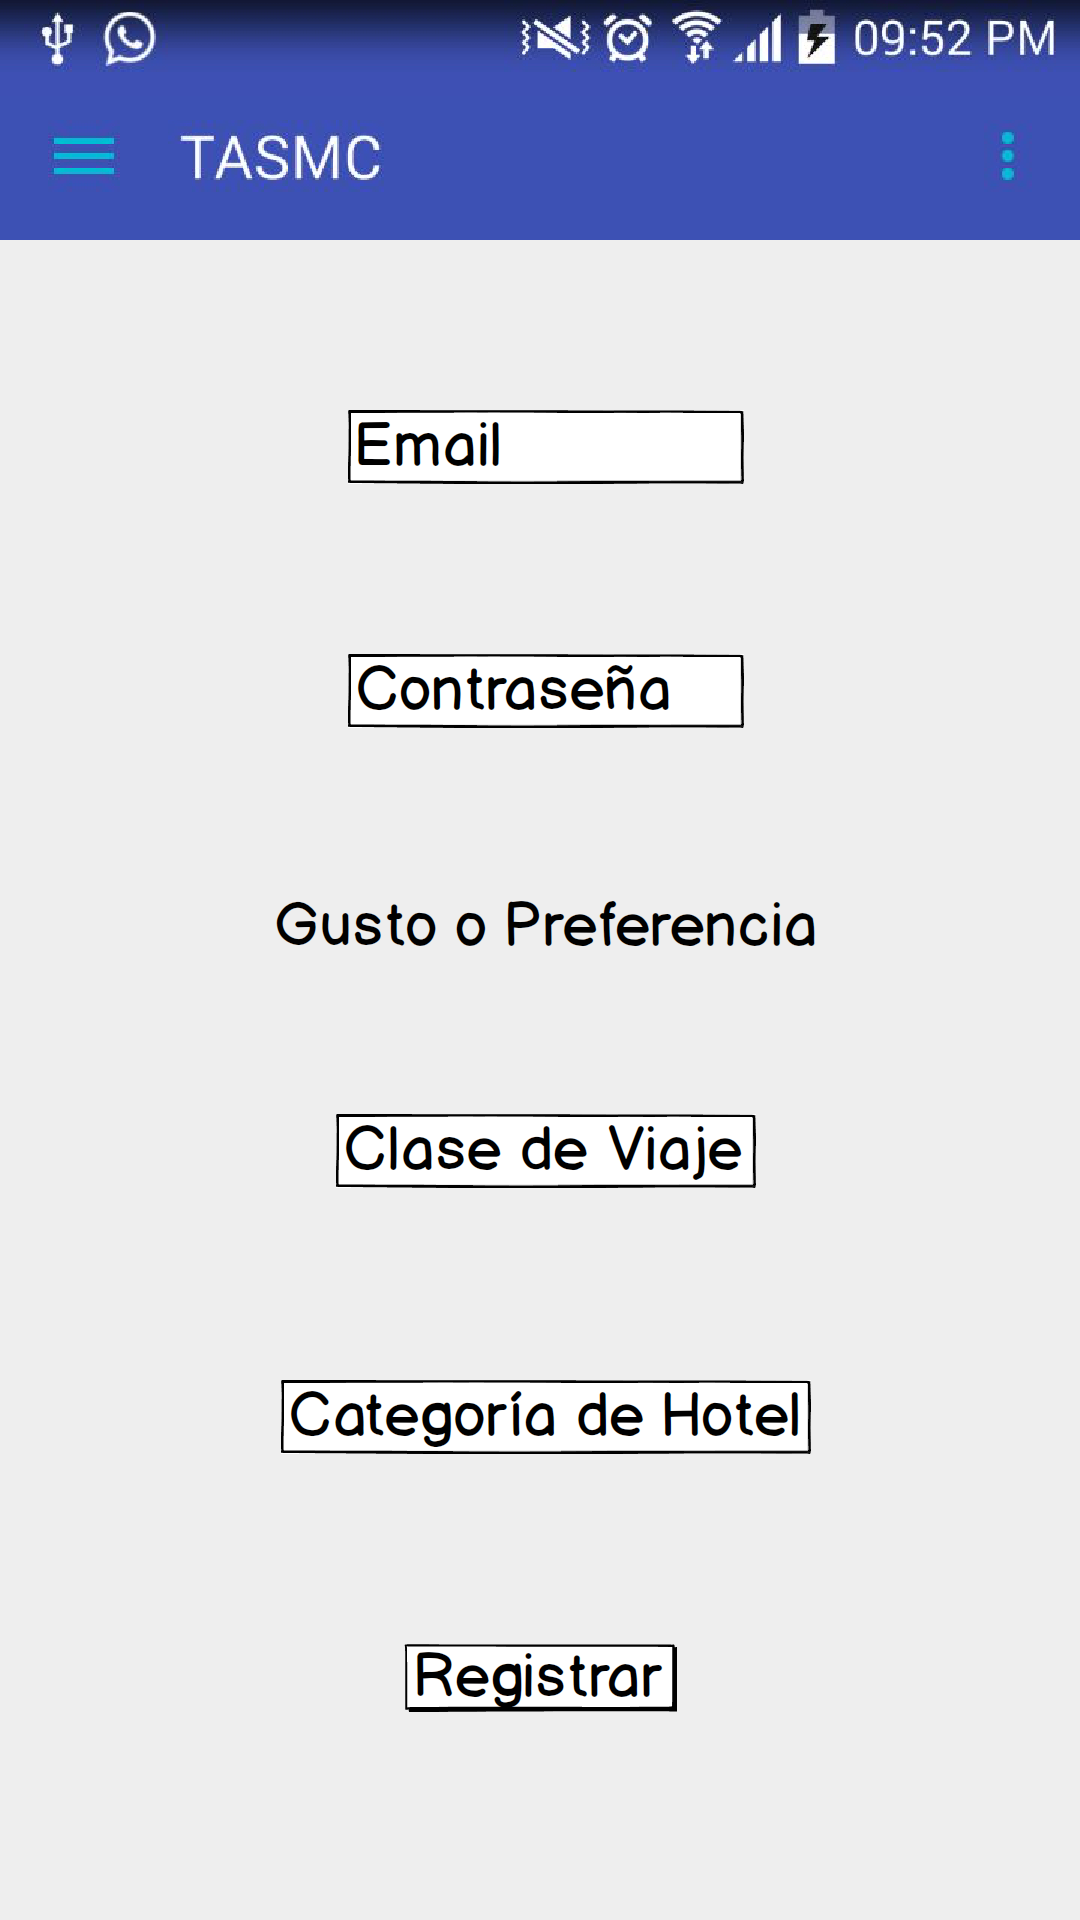
\includegraphics[width=0.4\textwidth]{Figuras/intConfiguracion.png}
		\rule{30em}{0.5pt}
	\caption[Pantalla configurar viaje]{Pantalla configurar viaje}
	\label{fig:intConfiguracion}
\end{figure}

\textbf{Descripción} \\
Los campos email y contraseña, se utilizan para el registro del usuario. Clase de viaje y categoría de hotel, requieren información que el usuario debe proporcionar para que la personalización de su viaje sea mejor. Finalmente, se obsera un botón que envia los datos del formulario a la aplicación web de TASMC. \\

\textbf{Entradas}
\begin{itemize}
\item Se escribe el email del usuario.
\item Se escribe la contraseña que el usuario utilizará para ingresar a los datos de TASMC.
\item Se escribe la clase en la cual el usuario prefiere al volar.
\item Se escribe la categoría de los hoteles que se prefieren. 
\end{itemize}

\textbf{Salidas}
\begin{itemize}
\item Se envian los datos a la base de datos.
\end{itemize}

\textbf{Controles}
\begin{itemize}
\item Botón Enviar, hará llegar la información al administrador.
\end{itemize}
\clearpage
\hypertarget{CU-U-02-1}{}
\subsection{Pantalla CU-U-02-1: Consultar Hotel}
\textbf{Objetivo}\\
Mostrar información de hoteles. \\

\textbf{Diseño:}
\begin{figure}[h]
	\centering
		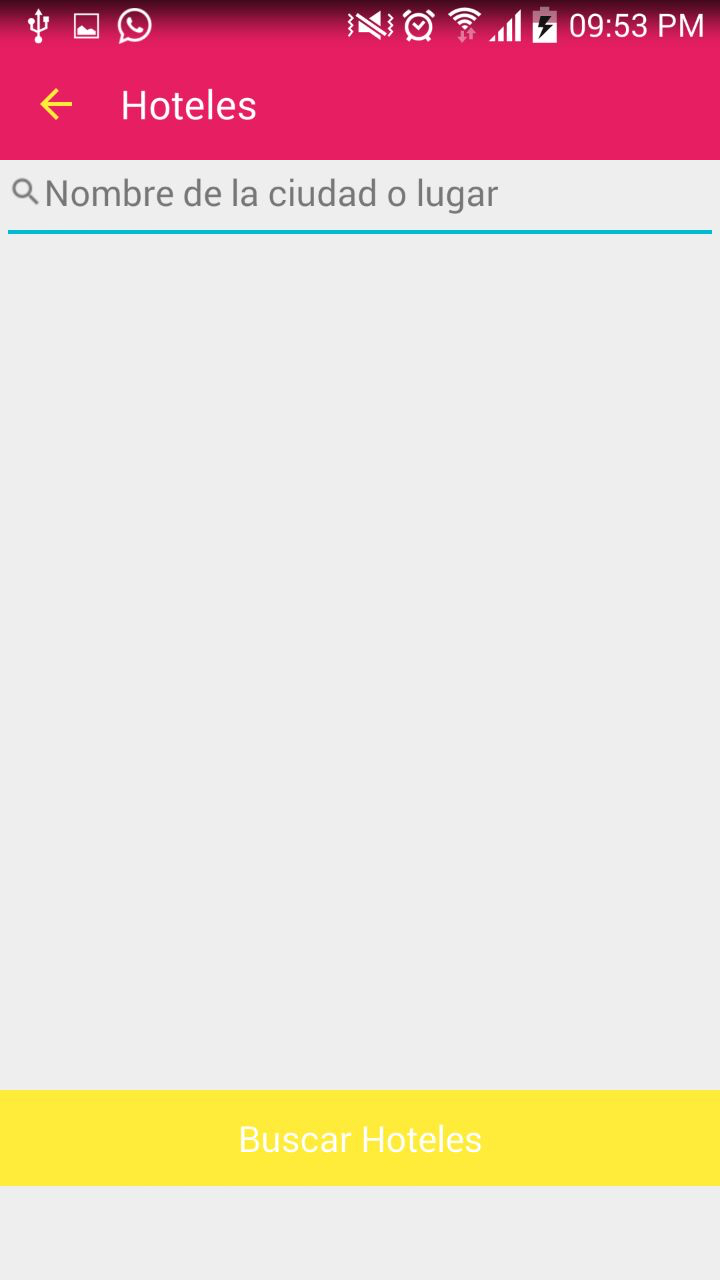
\includegraphics[width=0.4\textwidth]{Figuras/intHoteles.jpg}
		\rule{30em}{0.5pt}
	\caption[Pantalla consultar hotel]{Pantalla consultar hotel}
	\label{fig:intHoteles}
\end{figure}

\textbf{Descripción} \\
El campo "Nombre de la ciudad o lugar" es para ingresar la ciudad donde se estará buscando hotel y el botón "Buscar Hoteles" nos permite realizar la búsqueda utilizando como parámetro el nombre de la ciudad. \\

\textbf{Entradas}
\begin{itemize}
\item Se escribe la ciudad donde se alojará el usuario.
\end{itemize}

\textbf{Salidas}
\begin{itemize}
\item Se realiza la búsqueda del hotel.
\end{itemize}

\textbf{Controles}
\begin{itemize}
\item Botón Buscar Hoteles, permite realizar la búsqueda.
\end{itemize}
\clearpage
\hypertarget{CU-U-03-1}{}
\subsection{Pantalla CU-U-03-1: Consultar Vuelo}
\textbf{Objetivo}\\
Mostrar información de vuelos. \\

\textbf{Diseño:}
\begin{figure}[h]
	\centering
		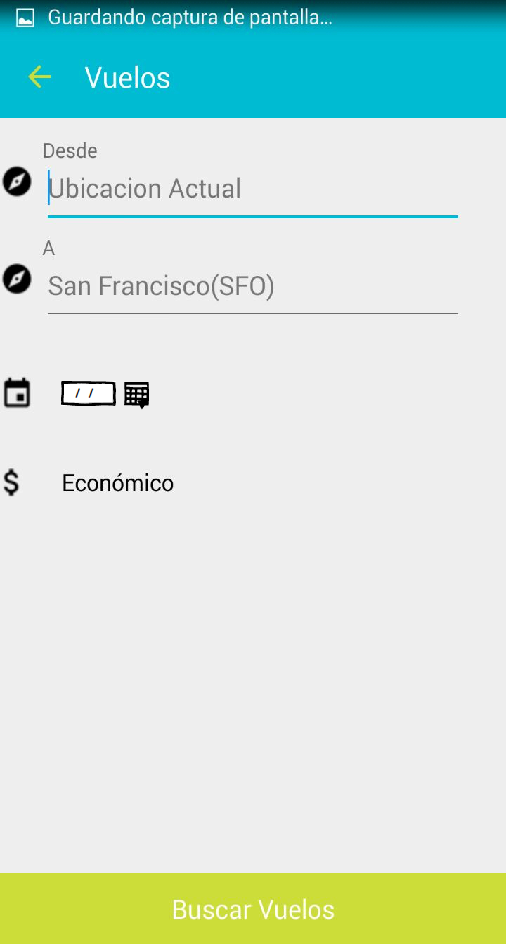
\includegraphics[width=0.4\textwidth]{Figuras/intConsultarVuelo.png}
		\rule{30em}{0.5pt}
	\caption[Pantalla consultar vuelo]{Pantalla consultar vuelo}
	\label{fig:intHoteles}
\end{figure}

\textbf{Descripción} \\
Los campos ``Desde'' y ``A'' son para ingresar la ciudad origen y destino del viaje. El siguiente campo es para ingresar la fecha de salida y, finalmente, se tiene un campo para ingresar la clase de vuelo que se busca. \\

\textbf{Entradas}
\begin{itemize}
\item Se escribe la ciudad origen.
\item Se escribe la ciudad destino.
\item Se ingresa la fecha de salida.
\item Se ingresa la clase de vuelo.
\end{itemize}

\textbf{Salidas}
\begin{itemize}
\item Se realiza la búsqueda del vuelo.
\end{itemize}

\textbf{Controles}
\begin{itemize}
\item Botón Buscar Vuelos, permite realizar la búsqueda.
\end{itemize}
\clearpage
\hypertarget{CU-U-04-1}{}
\subsection{Pantalla CU-U-04-1: Consultar Información AICM}
\textbf{Objetivo}\\
Mostrar información del AICM. \\

\textbf{Diseño:}
\begin{figure}[h]
	\centering
		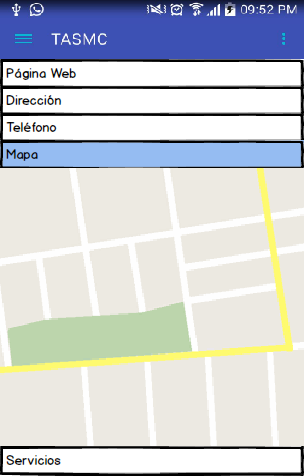
\includegraphics[width=0.4\textwidth]{Figuras/intConsultarInformacionAICM.png}
		\rule{30em}{0.5pt}
	\caption[Pantalla consultar información AICM]{Pantalla consultar información AICM}
	\label{fig:intConsultarInformacionAICM}
\end{figure}

\textbf{Descripción} \\
Es una pantalla con diferentes pestañas, cada una brinda información sobre el AICM. El teléfono, página web, dirección, mapa interior y Servicios, será la información que se pueda consultar. \\

\textbf{Entradas}
\begin{itemize}
\item Se elige una pestaña.
\end{itemize}

\textbf{Salidas}
\begin{itemize}
\item Se abre la pestaña elegida para visualizar la información que contiene.
\end{itemize}
\clearpage
\hypertarget{CU-U-05-1}{}
\subsection{Pantalla CU-U-05-1: Gestionar Equipaje}
\textbf{Objetivo}\\
Mostrar las listas de equipaje disponibles y las opciones de agregar, editar o eliminar una lista y/o sus objetos. \\

\textbf{Diseño:}
\begin{figure}[h]
	\centering
		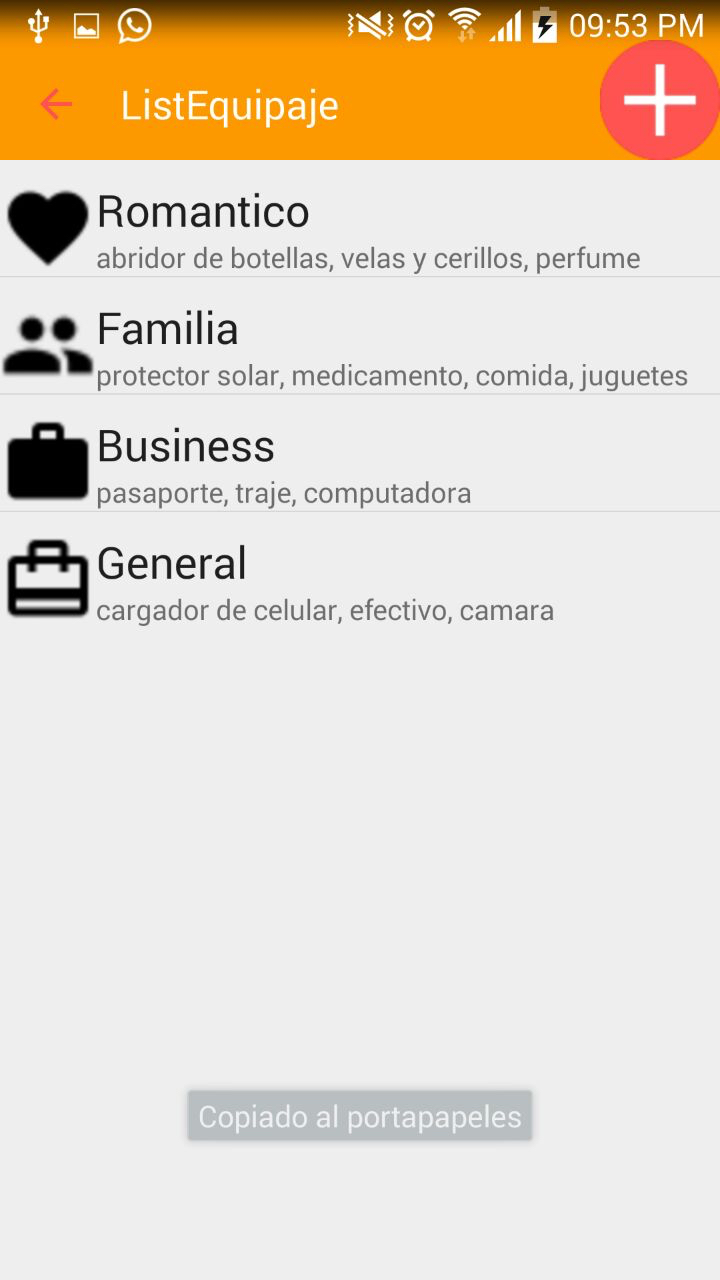
\includegraphics[width=0.4\textwidth]{Figuras/intListaEquipaje.jpg}
		\rule{30em}{0.5pt}
	\caption[Pantalla Equipaje]{Pantalla Equipaje}
	\label{fig:intListaEquipaje}
\end{figure}

\textbf{Descripción} \\
Se visualizan 4 listas predefinidas, el usuario puede abrir cualquiera para ver su contenido. También está el icono ``+'' el cual nos da la opción de crear una nueva lista. \\

\textbf{Entradas}
\begin{itemize}
\item Se elige una lista para visualizar su contenido.
\item Se elige crear una nueva lista.
\end{itemize}

\textbf{Salidas}
\begin{itemize}
\item Muestra un listado de objetos que son el contenido del equipaje elegido.
\end{itemize}

\textbf{Controles}
\begin{itemize}
\item Botón agregar, para ingresar una nueva lista de objetos.
\end{itemize}
\clearpage
\hypertarget{CU-U-06-1}{}
\subsection{Pantalla CU-U-06-1: Consultar Itinerario de Viaje}
\textbf{Objetivo}\\
Mostrar al usuario el itinerario de su viaje. \\

\textbf{Diseño:}
\begin{figure}[h]
	\centering
		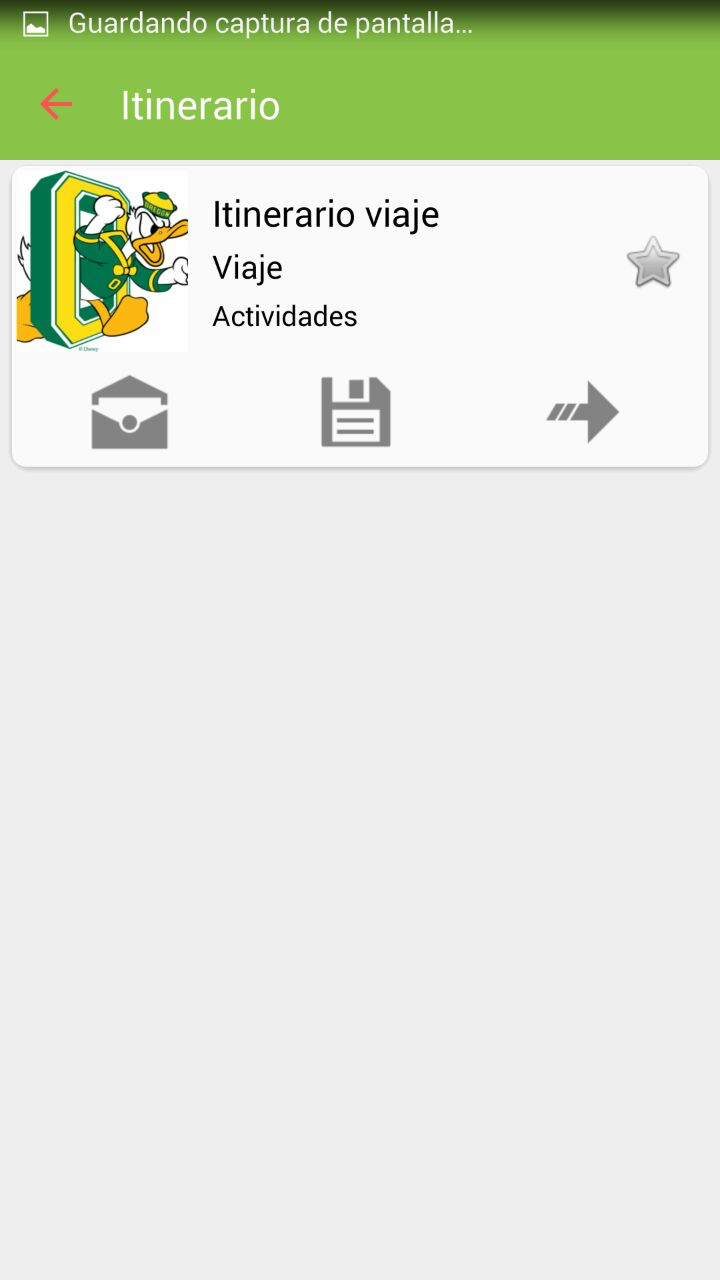
\includegraphics[width=0.4\textwidth]{Figuras/intItinerarioViaje.jpg}
		\rule{30em}{0.5pt}
	\caption[Pantalla Itinerario de Viaje]{Pantalla Itinerario de Viaje}
	\label{fig:intItinerarioViaje}
\end{figure}

\textbf{Descripción} \\
Se visualizan los botones para ingresar nuevas actividades, guardar el itinerario, visualizar el itinerario y poner como favorita cierta actividad. \\

\textbf{Entradas}
\begin{itemize}
\item Se elige una opción para ejecutar la acción de algún botón.
\end{itemize}

\textbf{Salidas}
\begin{itemize}
\item Muestra la tarea del botón elegido.
\end{itemize}

\textbf{Controles}
\begin{itemize}
\item Botón agregar, para ingresar una nueva actividad
\item Botón guardar, para actualzar el itinerario con las actividades nuevas.
\item Botón ver, para visualizar el itinerario.
\item Botón favorito, para marcar alguna actividad como favorito.
\end{itemize}
\clearpage
\hypertarget{CU-U-07-1}{}
\subsection{Pantalla CU-U-07-1: Consultar Ruta casa-AICM}
\textbf{Objetivo}\\
Mostrar la ruta para llegar al AICM \\

\textbf{Diseño:}
\begin{figure}[h]
	\centering
		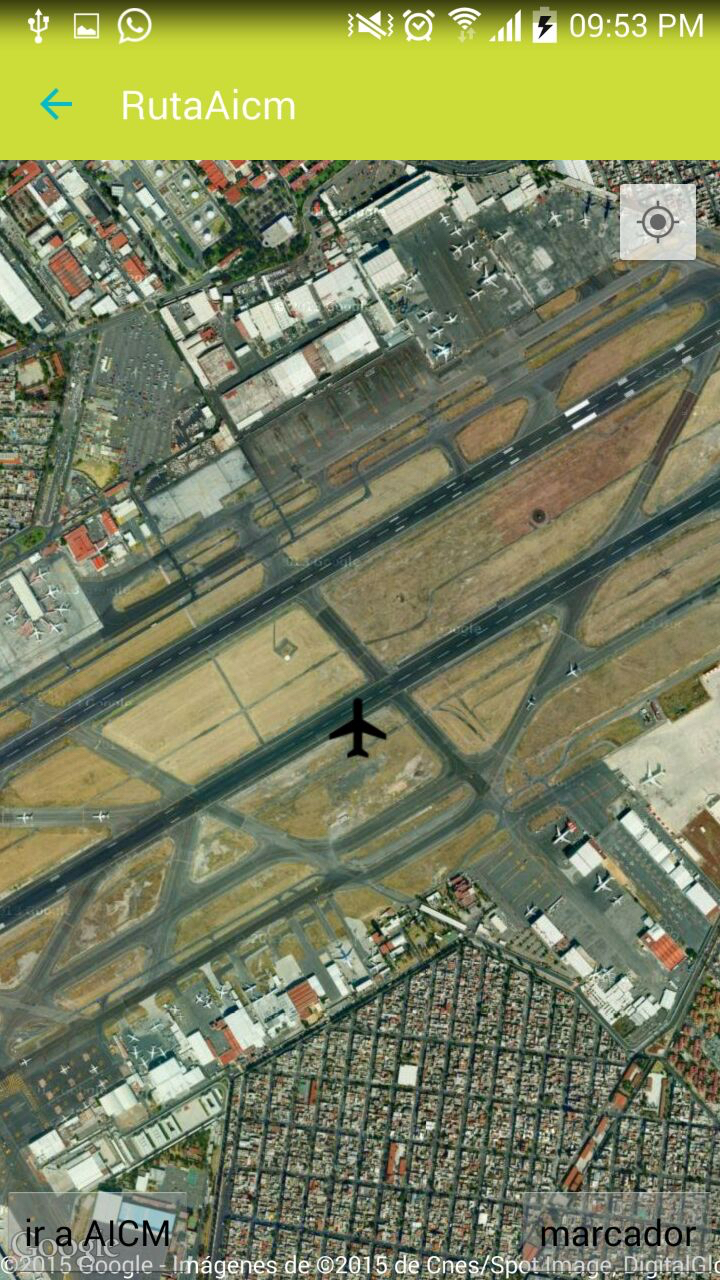
\includegraphics[width=0.4\textwidth]{Figuras/intRutaAICM.jpg}
		\rule{30em}{0.5pt}
	\caption[Pantalla Ruta AICM]{Pantalla Ruta AICM}
	\label{fig:intRutaAICM}
\end{figure}

\textbf{Descripción} \\
Se visualiza un mapa con la ruta desde el punto donde se encuentre el usuario hasta el AICM. \\

\textbf{Entradas}
\begin{itemize}
\item Se oprime el botón del menú para ingresar a la presente pantalla.
\end{itemize}

\textbf{Salidas}
\begin{itemize}
\item Muestra la presente pantalla con la ruta al AICM.
\end{itemize}

\textbf{Controles}
\begin{itemize}
\item Botón Ir a AICM, para generar la ruta al AICM.
\item Botón Marcador, para agregar algún marcador en el mapa.
\end{itemize}

\clearpage
\hypertarget{CU-U-08-1}{}
\subsection{Pantalla CU-U-08-1: Ubicar en AICM}
\textbf{Objetivo}\\
Apoyar al usuario para ubicarse dento del AICM. \\

\textbf{Diseño:}
\begin{figure}[h]
	\centering
		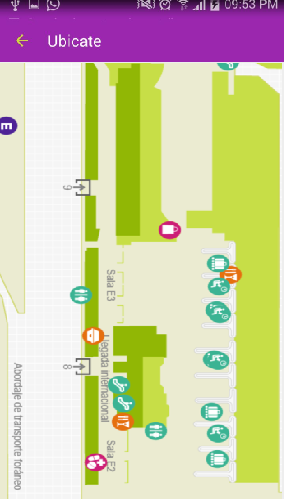
\includegraphics[width=0.4\textwidth]{Figuras/intUbicarAICM.png}
		\rule{30em}{0.5pt}
	\caption[Pantalla Ubicar en AICM]{Pantalla Ubicar en AICM}
	\label{fig:intUbicarAICM}
\end{figure}

\textbf{Descripción} \\
Se visualiza un mapa con el interior del AICM para que el usuario pueda ubicarse dentro del mismo y, de esa forma, no perderse mientras busca algún lugar de su interés. También podemos observar que se muestran los iconos de servicios en el AICM. \\

\textbf{Entradas}
\begin{itemize}
\item Se ingresa al mapa del AICM
\end{itemize}

\textbf{Salidas}
\begin{itemize}
\item Muestra el AICM y sus servicios según la zona donde se encuentre el usuario.
\end{itemize}
\clearpage
\hypertarget{CU-U-09-1}{}
\subsection{Pantalla CU-U-09-1: Consultar Información de Vuelo}
\textbf{Objetivo}\\
Permitir visualizar la información del vuelo en donde el usuario va a ingresar. \\

\textbf{Diseño:}
\begin{figure}[h]
	\centering
		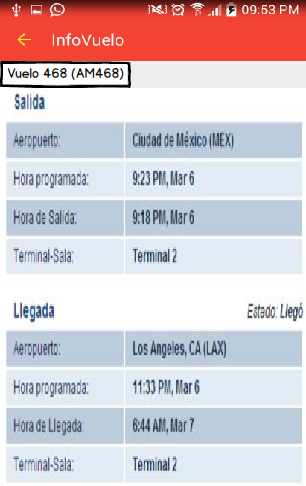
\includegraphics[width=0.4\textwidth]{Figuras/intInformacionVuelo.png}
		\rule{30em}{0.5pt}
	\caption[Pantalla Información del Vuelo]{Pantalla Información del Vuelo}
	\label{fig:intInformacionVuelo}
\end{figure}

\textbf{Descripción} \\
Se visualizan la información del vuelo del usuario. \\

\textbf{Entradas}
\begin{itemize}
\item Se oprime el botón del menú para ingresar a la presente pantalla.
\end{itemize}

\textbf{Salidas}
\begin{itemize}
\item Muestra la presente pantalla con la información del vuelo.
\end{itemize}